%File: sokrates.tex
\documentclass[letterpaper]{article} % DO NOT CHANGE THIS
\usepackage[submission]{aaai2026}  % DO NOT CHANGE THIS
\usepackage{times}  % DO NOT CHANGE THIS
\usepackage{helvet}  % DO NOT CHANGE THIS
\usepackage{courier}  % DO NOT CHANGE THIS
\usepackage[hyphens]{url}  % DO NOT CHANGE THIS
\usepackage{graphicx} % DO NOT CHANGE THIS
\urlstyle{rm} % DO NOT CHANGE THIS
\def\UrlFont{\rm}  % DO NOT CHANGE THIS
\usepackage{natbib}  % DO NOT CHANGE THIS AND DO NOT ADD ANY OPTIONS TO IT
\usepackage{caption} % DO NOT CHANGE THIS AND DO NOT ADD ANY OPTIONS TO IT
\frenchspacing  % DO NOT CHANGE THIS
\setlength{\pdfpagewidth}{8.5in} % DO NOT CHANGE THIS
\setlength{\pdfpageheight}{11in} % DO NOT CHANGE THIS
%
% Math packages (allowed for mathematics)
\usepackage{amsmath}
\usepackage{amssymb}
%
% TikZ for diagrams
\usepackage{tikz}
\usetikzlibrary{shapes, arrows.meta, positioning, calc, fit, backgrounds}
%
% These are recommended to typeset algorithms but not required.
\usepackage{algorithm}
\usepackage{algorithmic}
%
% These are recommended to typeset listings but not required.
\usepackage{newfloat}
\usepackage{listings}
\DeclareCaptionStyle{ruled}{labelfont=normalfont,labelsep=colon,strut=off} % DO NOT CHANGE THIS
\lstset{%
	basicstyle={\footnotesize\ttfamily},% footnotesize acceptable for monospace
	numbers=left,numberstyle=\footnotesize,xleftmargin=2em,% show line numbers
	aboveskip=0pt,belowskip=0pt,%
	showstringspaces=false,tabsize=2,breaklines=true}
\floatstyle{ruled}
\newfloat{listing}{tb}{lst}{}
\floatname{listing}{Listing}
%
\pdfinfo{
/TemplateVersion (2026.1)
}

\setcounter{secnumdepth}{0} %May be changed to 1 or 2 if section numbers are desired.

% Custom commands for this paper
\newcommand{\qhat}{\hat{q}_\phi}
\newcommand{\sokrates}{Sokrates}
\newcommand{\oak}{OaK}
\newcommand{\dpo}{DPO}

\title{SOKRATES: Distilling Symbolic Knowledge into Option-Level Reasoning via Solver-Guided Preference Optimization}
\author{
    Anonymous Submission
}
\affiliations{
    
}

\begin{document}

\maketitle

\begin{abstract}
Large language models (LLMs) frequently produce logically invalid chain-of-thought (CoT) reasoning even when their final answers are correct. 
Existing neuro-symbolic approaches improve consistency by enforcing logical constraints (LoCo-LMs) or verifying proofs post-hoc (Logic-LM), but they treat reasoning as unstructured text and do not explicitly model which reasoning actions are reliable in which contexts.
We introduce \sokrates{} (\textbf{S}ymbolic \textbf{O}ption-\textbf{K}nowledge \textbf{R}easoning \textbf{A}lignment via \textbf{T}race \textbf{E}valuation with \textbf{S}olver), a method that instantiates Sutton's \emph{Options and Knowledge} (\oak{}) framework in a first-order logic micro-world.
\sokrates{} represents proofs as sequences of discrete reasoning \textbf{options}---inference-rule macros such as \texttt{MODUS\_PONENS} or \texttt{UNIV\_INST}---rather than free-form tokens.
A FOL solver provides ground-truth \textbf{knowledge} by verifying each option application.
From solver feedback, we (i) train an explicit option-success predictor $\qhat(s,\omega)$ and (ii) construct preference pairs over optionized traces, applying Direct Preference Optimization (\dpo{}) to align the LLM's option policy.
Experiments on PrOntoQA show that \sokrates{} improves final accuracy, full-trace validity, and calibration of $\qhat$ compared to supervised fine-tuning, yielding a concrete \oak{}-style loop for symbolic reasoning.
\end{abstract}

%============================================================================
\section{Introduction}
%============================================================================

Large language models have demonstrated remarkable capabilities in multi-step reasoning through chain-of-thought (CoT) prompting \cite{wei2022chain} and decoding strategies such as self-consistency \cite{wang2023selfconsistency}.
However, even when LLMs produce correct final answers, their intermediate reasoning steps frequently contain logical errors, invalid inferences, and contradictions \cite{saparov2023language, huang2024large}.
This ``right answer, wrong reasoning'' phenomenon undermines the reliability of LLM-based reasoning systems.

Recent neuro-symbolic approaches address this gap through two main strategies.
\emph{Semantic loss methods} like LoCo-LMs \cite{riegel2020logical} add differentiable constraints encouraging token-level logical consistency, but do not model reasoning as structured actions.
\emph{Solver-verified CoT methods} like Logic-LM \cite{pan2023logic} and LINC \cite{olausson2023linc} parse reasoning into FOL and use solvers for verification, but focus on validating traces post-hoc rather than learning predictive models of which reasoning steps will succeed.
Recent test-time reasoning frameworks such as Tree-of-Thoughts \cite{yao2024tree} and Buffer-of-Thoughts \cite{yang2024buffer} improve search but still treat reasoning as unstructured text.

We argue that logical reasoning can be naturally formulated as a sequential decision problem where the agent selects \emph{which inference rule to apply} at each step.
This view aligns with Sutton's \emph{Options and Knowledge} (\oak{}) framework \cite{sutton2023reward}, which advocates for:
(1) \textbf{options}---temporally extended, reusable behaviors; and
(2) \textbf{knowledge}---explicit predictive models of how options behave.
We instantiate this program in a first-order logic micro-world by treating inference rules as options and the solver as a source of predictive knowledge about option success.

We make three contributions:

\begin{enumerate}
    \item \textbf{Optionized reasoning}: We represent proofs as sequences of discrete \emph{options}---inference-rule macros (e.g., \texttt{MODUS\_PONENS}, \texttt{UNIV\_INST}) with arguments---using a structured Thought/Action format.
    
    \item \textbf{Explicit option models}: We train an option-success predictor $\qhat(s,\omega)$ that estimates the probability a given option will be solver-valid in state $s$, providing explicit ``knowledge'' about reasoning actions.
    
    \item \textbf{Solver-guided \dpo{}}: We construct preference pairs where solver-valid traces are preferred over invalid ones, applying \dpo{} \cite{rafailov2023direct} to align the policy with solver-induced preferences.
\end{enumerate}

Figure~\ref{fig:architecture} gives an overview of the \sokrates{} \oak{} loop: generate optionized traces $\rightarrow$ verify with solver $\rightarrow$ update $\qhat$ and policy $\rightarrow$ repeat.
Experiments on PrOntoQA demonstrate that \sokrates{} improves both accuracy and full-trace validity while producing well-calibrated predictions of step validity.

% Architecture figure (moved to Introduction per improvement suggestions)
% figures/architecture.tex
% SOKRATES architecture diagram using TikZ

\begin{figure*}[t]
\centering
\resizebox{\textwidth}{!}{%
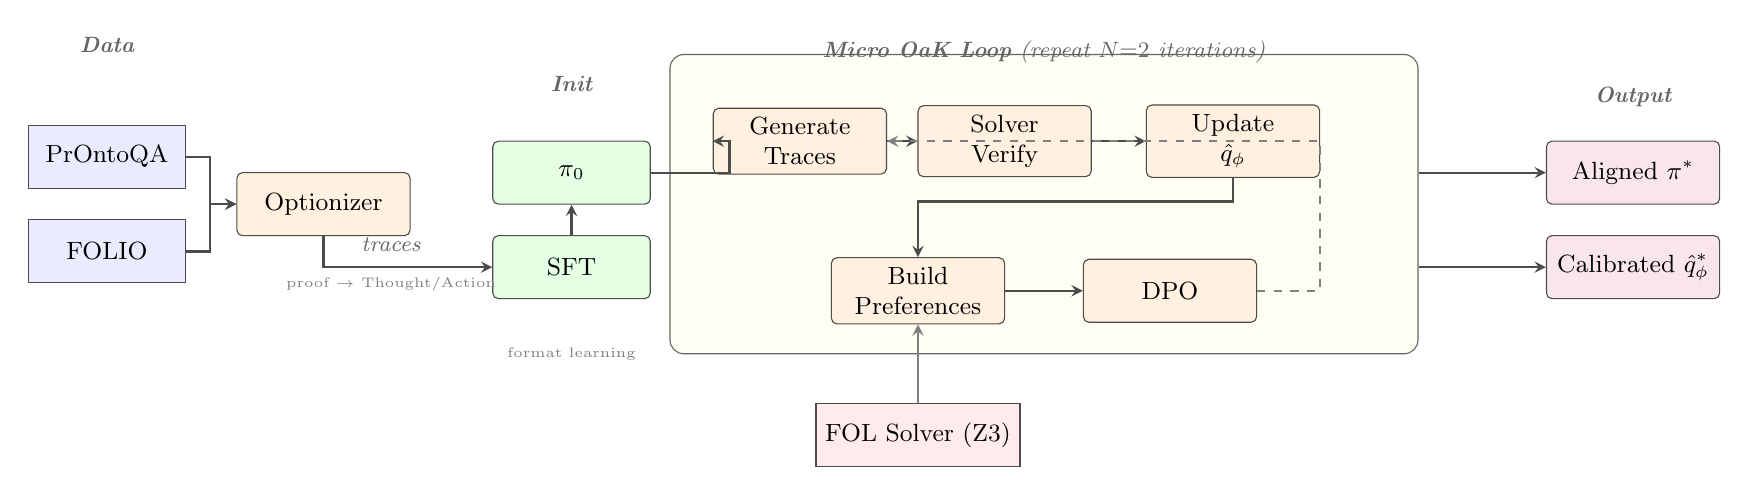
\begin{tikzpicture}[
    % Node styles
    data/.style={rectangle, draw=black!70, fill=blue!8, minimum width=2cm, minimum height=0.8cm, align=center, font=\small},
    process/.style={rectangle, draw=black!70, fill=orange!12, minimum width=2.2cm, minimum height=0.8cm, align=center, font=\small, rounded corners=2pt},
    model/.style={rectangle, draw=black!70, fill=green!10, minimum width=2cm, minimum height=0.8cm, align=center, font=\small, rounded corners=2pt},
    output/.style={rectangle, draw=black!70, fill=purple!10, minimum width=2.2cm, minimum height=0.8cm, align=center, font=\small, rounded corners=2pt},
    loopbox/.style={rectangle, draw=black!60, fill=yellow!5, rounded corners=5pt, inner sep=8pt},
    arrow/.style={->, >=stealth, thick, black!70},
    looparrow/.style={->, >=stealth, thick, black!50, dashed},
    label/.style={font=\footnotesize\itshape, text=black!60},
]

% === LEFT: Data Sources ===
\node[data] (prontoqa) at (-0.4, 1.0) {PrOntoQA};
\node[data] (folio) at (-0.4, -0.2) {FOLIO};
\node[process] (optionizer) at (2.35, 0.4) {Optionizer};

% === CENTER-LEFT: SFT ===
\node[model] (sft) at (5.5, -0.4) {SFT};
\node[model] (pi0) at (5.5, 0.8) {$\pi_0$};

% === CENTER: OaK Loop ===
\begin{scope}[shift={(11.5, 0.4)}]
    % Loop background
    \node[loopbox, minimum width=9.5cm, minimum height=3.8cm] (loopbg) at (0, 0) {};
    \node[label, anchor=north] at (0, 2.2) {\textbf{Micro \oak{} Loop} (repeat $N{=}2$ iterations)};
    
    % Loop nodes
    \node[process] (generate) at (-3.1, 0.8) {Generate\\Traces};
    \node[process] (verify) at (-0.5, 0.8) {Solver\\Verify};
    \node[process] (qhat) at (2.4, 0.8) {Update\\$\qhat$};
    \node[process] (prefs) at (-1.6, -1.1) {Build\\Preferences};
    \node[process] (dpo) at (1.6, -1.1) {DPO};
    
    % Loop arrows
    \draw[arrow] (generate) -- (verify);
    \draw[arrow] (verify) -- (qhat);
    \draw[arrow] (qhat.south) -- ++(0, -0.3) -| (prefs.north);
    \draw[arrow] (prefs) -- (dpo);
    \draw[looparrow] (dpo.east) -- ++(0.8, 0) |- (generate.east);
\end{scope}

% === RIGHT: Outputs (aligned on a common x, tied to loop)
\node[right=2.6cm of loopbg.east] (output_anchor) {};
\node[output] (pistar) at (output_anchor |- pi0) {Aligned $\pi^*$};
\node[output] (qhatstar) at (output_anchor |- sft) {Calibrated $\qhat^*$};

% === Solver (external, positioned relative to loop) ===
\node[data, fill=red!8, below=1.0cm of prefs] (solver) {FOL Solver (Z3)};

% === Main Flow Arrows (all relative) ===
\draw[arrow] (prontoqa.east) -- ++(0.3, 0) |- (optionizer.west);
\draw[arrow] (folio.east) -- ++(0.3, 0) |- (optionizer.west);
\draw[arrow] (optionizer.south) |- node[pos=0.7, above, label, yshift=2pt] {traces} node[pos=0.7, below, font=\tiny, text=black!50] {proof $\rightarrow$ Thought/Action} (sft.west);
\draw[arrow] (sft) -- (pi0);
\draw[arrow] (pi0.east) -- ++(1.0, 0) |- (generate.west);

% Arrow from loop to outputs (relative to nodes)
\draw[arrow] (loopbg.east |- pistar) -- (pistar.west);
\draw[arrow] (loopbg.east |- qhatstar) -- (qhatstar.west);

% Solver connection (relative to nodes)
\draw[arrow, black!50] (solver.north) -- (prefs.south);

% === Labels (relative to nodes) ===
\node[label, above=0.8cm of prontoqa] {\textbf{Data}};
\node[label, above=0.5cm of pi0] {\textbf{Init}};
\node[label, above=0.3cm of pistar] {\textbf{Output}};

% Annotations (relative to nodes)
\node[font=\tiny, text=black!50, below=0.5cm of sft] {format learning};

\end{tikzpicture}
}%
\caption{\sokrates{} architecture. \textbf{Left:} PrOntoQA/FOLIO problems are converted to optionized Thought/Action traces. \textbf{Center:} After SFT initialization, the micro \oak{} loop iterates: (1) generate traces from current policy, (2) verify each step with the FOL solver, (3) update the option-success predictor $\qhat$, (4) construct preference pairs, and (5) apply \dpo{} to improve the policy. \textbf{Right:} Final outputs are an aligned policy $\pi^*$ and a calibrated knowledge head $\qhat^*$.}
\label{fig:architecture}
\end{figure*}


%============================================================================
\section{Background and Related Work}
%============================================================================

\subsection{LLM Reasoning and Failure Modes}

Chain-of-thought prompting \cite{wei2022chain} and self-consistency decoding \cite{wang2023selfconsistency} are the current workhorses for LLM reasoning, but they do not guarantee logically valid chains.
Systematic analyses reveal that LLMs are \emph{greedy reasoners}---locally good at individual deductions but poor at proof planning when many valid next steps exist \cite{saparov2023language}.
Furthermore, self-reflection without external feedback often fails to fix logical errors \cite{huang2024large}.

\sokrates{} tackles exactly this ``right answer, wrong reasoning'' regime by explicitly modeling which \emph{optionized} reasoning actions are solver-valid in which states, rather than relying on the surface plausibility of free-form thoughts.

\subsection{Logical Reasoning Benchmarks}

\paragraph{Synthetic Benchmarks.}
RuleTaker and ProofWriter \cite{clark2021transformers} provide synthetic rule-based reasoning with multi-hop proofs.
PrOntoQA \cite{saparov2023language} offers first-order synthetic worlds with formally analyzable CoT, making it ideal for isolating reasoning behavior.

\paragraph{Natural Language Benchmarks.}
FOLIO \cite{han2022folio} provides natural language premises with expert FOL annotations.
P-FOLIO extends it with human-written proof chains labeled with inference rules, which inform our option vocabulary.

We choose PrOntoQA as our primary testbed because it provides ground-truth proofs and fully specified FOL world models, enabling us to parse and verify every optionized step with a solver.

\subsection{Neuro-Symbolic Methods and Solver-Augmented Reasoning}

Prior work on integrating symbolic reasoning with LLMs falls into three categories:

\paragraph{LM + External Solver at Inference.}
LINC \cite{olausson2023linc} uses LLMs as semantic parsers to generate FOL, with external provers computing answers.
Logic-LM \cite{pan2023logic} parses CoT into FOL for solver verification and uses error messages for self-refinement.
LAMBADA \cite{kazemi2022lambada} employs backward-chaining control with LLM modules.
These approaches ``outsource'' proof search to symbolic engines but do not train an internal option model.

\paragraph{LMs Trained to Simulate Solvers.}
LoGiPT \cite{feng2024logipt} trains an LM on hidden intermediate steps of a deductive solver; the LM emulates the solver and can answer without external calls.
Unlike \sokrates{}, LoGiPT trains on full solver traces but does not decompose them into reusable option macros or learn a separate predictive head for step validity.

\paragraph{Neuro-Symbolic Consistency Objectives.}
LoCo-LMs and Logical Neural Networks \cite{riegel2020logical} incorporate differentiable logic constraints via semantic loss functions, encouraging consistency at the prediction level.
These operate on truth values or soft logical constraints, not on a structured sequence of options with explicit per-option success probabilities.

\paragraph{Positioning \sokrates{}.}
\sokrates{} is closest in spirit to Logic-LM and LoGiPT, in that it uses a symbolic solver to supervise reasoning, but differs by:
(i) factorizing reasoning into a finite option vocabulary,
(ii) learning an explicit option-success model $\qhat(s,\omega)$, and
(iii) using solver-derived preferences to shape an option policy via \dpo{} rather than directly imitating solver traces.

\subsection{Preference Learning and Process Supervision}

Direct Preference Optimization (\dpo{}) \cite{rafailov2023direct} provides an efficient alternative to PPO-style RLHF \cite{ouyang2022training} and has been widely adopted for LLM alignment.
Given preference pairs $(y_w, y_l)$ where $y_w$ is preferred over $y_l$, \dpo{} optimizes:
\begin{equation}
\mathcal{L}_{\text{DPO}} = -\mathbb{E}\left[\log \sigma\left(\beta \log \frac{\pi_\theta(y_w|x)}{\pi_{\text{ref}}(y_w|x)} - \beta \log \frac{\pi_\theta(y_l|x)}{\pi_{\text{ref}}(y_l|x)}\right)\right]
\label{eq:dpo}
\end{equation}
where $\pi_{\text{ref}}$ is a reference policy and $\beta$ controls the KL penalty.

\paragraph{Verifier-Based Preferences.}
VeriCoT \cite{ling2023deductive} translates CoT to FOL, verifies each step with a solver, and uses verification-based preferences for fine-tuning.
However, VeriCoT operates on \textbf{unstructured CoT text}, using a parser to extract predicates.
\sokrates{} instead uses a fixed \textbf{finite option set} with typed arguments (Table~\ref{tab:options}), trains an explicit knowledge head $\qhat(s,\omega)$ parallel to \dpo{}, and frames this as a micro \oak{} loop where option models are learned as predictive knowledge.

\subsection{Options, OaK, and Hierarchical RL}

The classic \textbf{options} framework \cite{sutton1999between} defines options as temporally extended actions with an initiation set, intra-option policy, and termination condition, enabling temporal abstraction and planning.

The \oak{} framework \cite{sutton2023reward} extends this by emphasizing that agents should learn not just policies but also \textbf{knowledge}---predictive models of how options behave.
\oak{} advocates \emph{reward-respecting subtasks} whose optimal policies do not conflict with the main objective.

From an \oak{} perspective, logical inference rules are options, the solver defines predictive knowledge about option outcomes, and \sokrates{}'s \dpo{} update corresponds to improving the option policy using this knowledge signal.
Importantly, our ``maintain logical consistency while answering the query'' subtask is reward-respecting: the main reward is correctness; the subtask reward is solver-validated step correctness; they are aligned, not competing.

%============================================================================
\section{Problem Setup: OaK in a Logic World}
%============================================================================

We formulate logical reasoning as a sequential decision problem where an agent selects and applies inference rules to derive a conclusion.

\subsection{States and Goals}

A \textbf{logical state} $s$ consists of:
\begin{itemize}
    \item $\mathcal{P} = \{p_1, \ldots, p_n\}$: premises (natural language + FOL)
    \item $\mathcal{D} = \{d_1, \ldots, d_k\}$: derived formulas from previous steps
    \item $c$: the target conclusion
\end{itemize}

The \textbf{goal} is to determine whether $c$ is \textsc{True}, \textsc{False}, or \textsc{Unknown}.

\subsection{Options as Inference Rules}

We define a finite \textbf{option vocabulary} $\Omega$ of inference-rule macros (Table~\ref{tab:options}).
These 11 rules cover all proof chains in our PrOntoQA variant; we leave option discovery as future work.

Although each option is invoked in a single decision step, it spans multiple sub-operations: choosing the rule type, selecting premise indices, generating a natural-language justification, and updating the proof state.
Thus, options function as \emph{temporally extended cognitive macros} in the \oak{} sense.

% Option vocabulary table (modular)
% tables/options.tex
% Option vocabulary table

\begin{table}[t]
\centering
{\small
\setlength{\tabcolsep}{3pt}
\renewcommand{\arraystretch}{0.95}
\begin{tabular}{@{}p{0.40\columnwidth}c c p{0.34\columnwidth}@{}}
\hline
\textbf{Option} & \textbf{Sym.} & \textbf{Args} & \textbf{Rule} \\
\hline
\texttt{MODUS\_\allowbreak PONENS} & MP & $(i, j)$ & $P, P{\rightarrow}Q \vdash Q$ \\
\texttt{MODUS\_\allowbreak TOLLENS} & MT & $(i, j)$ & $\neg Q, P{\rightarrow}Q \vdash \neg P$ \\
\texttt{UNIV\_\allowbreak INSTANTIATION} & UI & $(i, c)$ & $\forall x.P(x) \vdash P(c)$ \\
\texttt{EXIST\_\allowbreak GENERALIZATION} & EG & $(i, x)$ & $P(c) \vdash \exists x.P(x)$ \\
\texttt{AND\_INTRO} & $\land$I & $(i, j)$ & $P, Q \vdash P \land Q$ \\
\texttt{AND\_ELIM} & $\land$E & $(i, s)$ & $P \land Q \vdash P$ or $Q$ \\
\texttt{OR\_INTRO} & $\lor$I & $(i, j)$ & $P \vdash P \lor Q$ \\
\texttt{DISJUNCTIVE\_\allowbreak SYLLOGISM} & DS & $(i, j)$ & $P{\lor}Q, \neg P \vdash Q$ \\
\texttt{HYPOTHETICAL\_\allowbreak SYLLOGISM} & HS & $(i, j)$ & $P{\rightarrow}Q, Q{\rightarrow}R \vdash P{\rightarrow}R$ \\
\texttt{DOUBLE\_\allowbreak NEGATION} & DN & $(i)$ & $\neg\neg P \vdash P$ \\
\texttt{CONCLUDE} & --- & $(l)$ & \parbox{0.95\linewidth}{Terminal: 0=True,\\ \mbox{1=False, 2=Unknown}} \\
\hline
\end{tabular}
}
\caption{Option vocabulary. These inference-rule macros cover the proof patterns in PrOntoQA.}
\label{tab:options}
\end{table}


\subsection{Knowledge: Solver as Ground Truth}

For each option application $\omega$ in state $s$, a \textbf{FOL solver} returns:
\begin{equation}
    \textsc{Solver}(s, \omega) = \begin{cases}
        (\textsc{Valid}, d') & \text{if } \omega \text{ is logically valid} \\
        (\textsc{Invalid}, \emptyset) & \text{otherwise}
    \end{cases}
    \label{eq:solver}
\end{equation}

This provides ground-truth ``knowledge'' for (1) training $\qhat$ and (2) constructing \dpo{} preferences.

\subsection{Thought/Action Format}

Following ReAct \cite{yao2023react}, each proof step is a \textbf{Thought/Action} pair.
Figure~\ref{fig:trace_example} shows a complete example trace with solver annotations.

% Trace example figure (modular)
% figures/trace_example.tex
% Example optionized proof trace with solver annotations

\begin{figure}[t]
\centering
\footnotesize
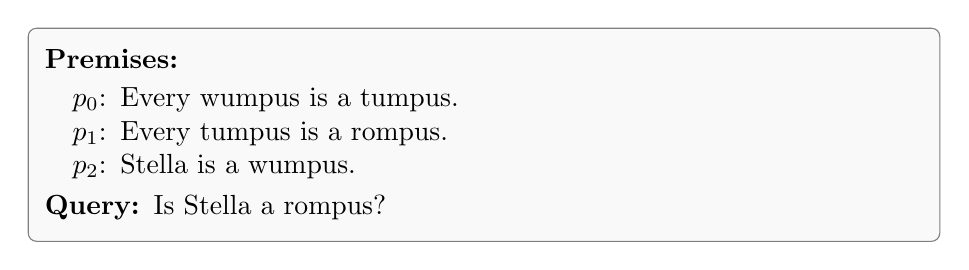
\begin{tikzpicture}
\node[draw=black!50, rounded corners=3pt, fill=gray!5, inner sep=6pt, text width=0.92\columnwidth] {
\begin{tabular}{@{}l@{}}
\textbf{Premises:}\\[2pt]
\hspace{1em}$p_0$: Every wumpus is a tumpus.\\
\hspace{1em}$p_1$: Every tumpus is a rompus.\\
\hspace{1em}$p_2$: Stella is a wumpus.\\[3pt]
\textbf{Query:} Is Stella a rompus?\\
\end{tabular}
};
\end{tikzpicture}

\vspace{0.4em}
\rule{0.92\columnwidth}{0.4pt}
\vspace{0.3em}

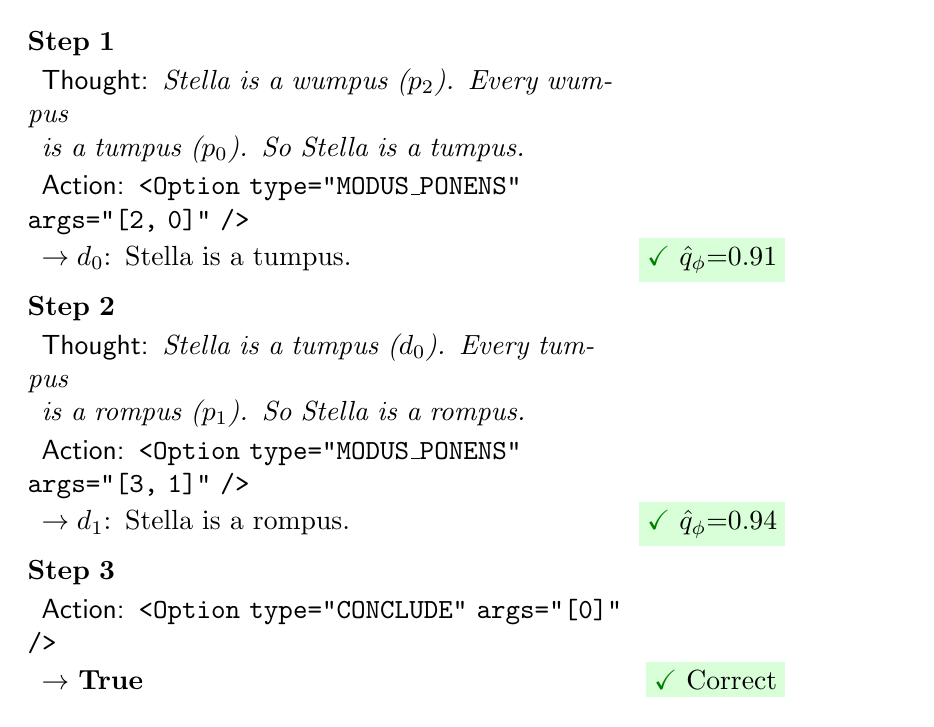
\begin{tikzpicture}
\node[text width=0.92\columnwidth, inner sep=0pt] {
\begin{tabular}{@{}p{0.68\columnwidth}@{\hspace{0.5em}}r@{}}
\textbf{Step 1} & \\[2pt]
\hspace{0.5em}\textsf{Thought:} \textit{Stella is a wumpus ($p_2$). Every wumpus} & \\
\hspace{0.5em}\textit{is a tumpus ($p_0$). So Stella is a tumpus.} & \\[2pt]
\hspace{0.5em}\textsf{Action:} \texttt{<Option type="MODUS\_PONENS" args="[2, 0]" />} & \\[2pt]
\hspace{0.5em}$\rightarrow d_0$: Stella is a tumpus. & \colorbox{green!15}{{\color{green!50!black}\checkmark} $\qhat{=}0.91$} \\[6pt]

\textbf{Step 2} & \\[2pt]
\hspace{0.5em}\textsf{Thought:} \textit{Stella is a tumpus ($d_0$). Every tumpus} & \\
\hspace{0.5em}\textit{is a rompus ($p_1$). So Stella is a rompus.} & \\[2pt]
\hspace{0.5em}\textsf{Action:} \texttt{<Option type="MODUS\_PONENS" args="[3, 1]" />} & \\[2pt]
\hspace{0.5em}$\rightarrow d_1$: Stella is a rompus. & \colorbox{green!15}{{\color{green!50!black}\checkmark} $\qhat{=}0.94$} \\[6pt]

\textbf{Step 3} & \\[2pt]
\hspace{0.5em}\textsf{Action:} \texttt{<Option type="CONCLUDE" args="[0]" />} & \\[2pt]
\hspace{0.5em}$\rightarrow$ \textbf{\textsc{True}} & \colorbox{green!15}{{\color{green!50!black}\checkmark} Correct} \\
\end{tabular}
};
\end{tikzpicture}
\caption{Example optionized proof trace. Each step includes a natural language \textsf{Thought}, a structured \textsf{Action} (option with arguments), the derived formula, and solver validity with $\qhat$ prediction.}
\label{fig:trace_example}
\end{figure}


%============================================================================
\section{Method: \sokrates{}}
%============================================================================

\sokrates{} consists of three components run in an iterative \oak{} loop (Algorithm~\ref{alg:oak}).

\subsection{Optionized Trace Generation}

Given problem $(s_0, c)$, we sample traces from policy $\pi_\theta$:

\begin{enumerate}
    \item Construct prompt with premises and target conclusion
    \item For $t = 1, \ldots, T_{\max}$:\footnote{We use $T_{\max}=6$ in our experiments due to computational constraints; the full design uses $T_{\max}=15$.}
    \begin{enumerate}
        \item Generate \texttt{Thought} via unconstrained sampling
        \item Generate \texttt{Action} via constrained decoding (grammar-guided to ensure valid option syntax)
        \item Parse option $\omega_t$, update state $s_{t+1}$
        \item Terminate if $\omega_t = \texttt{CONCLUDE}$ or no valid options remain
    \end{enumerate}
    \item Return trace $\tau = (s_0, \omega_1, s_1, \ldots, \omega_T, s_T)$
\end{enumerate}

Constrained decoding separates \emph{syntax errors} (eliminated by grammar) from \emph{semantic errors} (detected by solver).
SFT teaches the model valid Thought/Action syntax and the option vocabulary; it does \emph{not} guarantee logically correct reasoning.

\paragraph{Prompt Structure.}
We use a structured prompt that explicitly instructs the model to produce Thought/Action pairs with our option vocabulary (see Appendix~\ref{app:prompt} for the complete template).
Key design choices include:
\begin{itemize}
    \item \textbf{Numbered premises} enable options to reference formulas by index
    \item \textbf{Explicit rule vocabulary} in prompt constrains the option space
    \item \textbf{Terminal encoding} (0/1/2 for True/False/Unknown) provides unambiguous answer format
\end{itemize}

\subsection{Solver Verification}

For each trace $\tau$, we verify every step:
\begin{equation}
    v_t = \mathbf{1}[\textsc{Solver}(s_{t-1}, \omega_t) = \textsc{Valid}]
    \label{eq:step_valid}
\end{equation}

A trace is \textbf{fully valid} if all steps pass and the answer is correct:
\begin{equation}
    V(\tau) = \mathbf{1}\left[\left(\textstyle\prod_{t=1}^{T} v_t = 1\right) \land (\text{answer}(\tau) = \text{label})\right]
    \label{eq:trace_valid}
\end{equation}

\subsection{Option Success Predictor ($\qhat$)}

We train an \textbf{option-success head} $\qhat(s, \omega)$ predicting whether option $\omega$ will be solver-valid in state $s$:
\begin{equation}
    \qhat(s, \omega) = \sigma\left(\text{MLP}\left([\mathbf{h}_s; \mathbf{e}_\omega]\right)\right)
    \label{eq:qhat}
\end{equation}
where $\mathbf{h}_s$ is the LLM's hidden state and $\mathbf{e}_\omega$ is a learned option embedding.

Training uses binary cross-entropy on solver labels:
\begin{equation}
    \mathcal{L}_{\qhat} = -\mathbb{E}_{(s,\omega,v)}\left[v \log \qhat + (1{-}v) \log(1{-}\qhat)\right]
    \label{eq:qhat_loss}
\end{equation}

This head provides explicit ``knowledge'' about option reliability, evaluated via Brier score and ECE (Expected Calibration Error).

\subsection{Preference Pair Construction}

From verified traces, we construct \dpo{} preferences.
For each problem with $K$ sampled traces,\footnote{We use $K=2$ samples per problem due to computational constraints; the full design uses $K=8$.} we score each trace:
\begin{equation}
    \text{score}(\tau) = \frac{|\{t : v_t = 1\}|}{T} + \mathbf{1}[\text{correct}] + 0.5 \cdot \mathbf{1}[V(\tau) = 1]
    \label{eq:score}
\end{equation}
where the first term is the step validity rate, the second rewards correct final answers, and the third rewards fully valid traces.

\begin{itemize}
    \item \textbf{Winner} $\tau_w$: highest-scoring trace (ideally: correct answer + all steps valid)
    \item \textbf{Loser} $\tau_l$: lower-scoring trace (wrong answer or invalid steps)
\end{itemize}

Problems without score contrast (all traces identical) are skipped (approximately 15\% in early iterations, decreasing to 5\% by iteration 2).

\subsection{Micro \oak{} Loop}

We run $N=2$ iterations (Algorithm~\ref{alg:oak}):\footnote{Due to computational constraints, we use a time-optimized configuration: 2 \oak{} iterations (vs.\ 3 in the full design), 2 samples/problem (vs.\ 8), and greedy decoding for deterministic generation.}

% Training loop algorithm (modular)
% algorithms/oak_loop.tex
% SOKRATES training loop algorithm

\begin{algorithm}[tb]
\caption{\sokrates{} Training Loop}
\label{alg:oak}
\textbf{Input}: SFT model $\pi_0$, problems $\mathcal{P}$, solver\\
\textbf{Output}: Aligned model $\pi^*$, option head $\qhat^*$
\begin{algorithmic}[1]
\FOR{iteration $i = 1, \ldots, N$}
    \STATE \textbf{Generate:} Sample $K$ traces/problem from $\pi_{i-1}$ (ours: $K{=}2$)
    \STATE \textbf{Verify:} Label each step with solver (Eq.~\ref{eq:step_valid})
    \STATE \textbf{Update $\qhat$:} Train option head (Eq.~\ref{eq:qhat_loss})
    \STATE \textbf{Build preferences:} Construct $(\tau_w, \tau_l)$ pairs
    \STATE \textbf{\dpo{}:} Update $\pi_{i-1} \rightarrow \pi_i$ (Eq.~\ref{eq:dpo})
\ENDFOR
\STATE \textbf{return} $\pi_N$, $\qhat$
\end{algorithmic}
\end{algorithm}



This constitutes a ``baby \oak{}'' cycle: \emph{experience} (traces) $\rightarrow$ \emph{knowledge} (solver labels, $\qhat$) $\rightarrow$ \emph{policy improvement} (\dpo{}) $\rightarrow$ repeat.
\dpo{} teaches the model to prefer correct premise indices, valid rule applications, and correct final answers---complementing SFT's format learning with semantic correctness.

%============================================================================
\section{Experimental Setup}
%============================================================================

\subsection{Datasets}

\paragraph{PrOntoQA.}
We use the LoGiPT \cite{feng2024logipt} version containing 14,346 training and 1,594 test problems with proof depths 1--5 and varying distractors.

\paragraph{FOLIO.}
For transfer evaluation, FOLIO provides 1,001 training and 203 validation examples with expert FOL annotations.

\paragraph{Two-Phase Data Strategy.}
We employ different data scales for each training phase:
\begin{itemize}
    \item \textbf{SFT}: Full training set ($n{=}14{,}346$) to maximize format learning diversity
    \item \textbf{\sokrates{} loop}: Representative subset ($n{=}1{,}500$; 10\%) for efficient preference learning
\end{itemize}
This reflects a realistic deployment scenario: supervised data is abundant, but preference labels require expensive solver verification. 
Prior work on \dpo{}~\cite{rafailov2023direct} demonstrates that preference learning is sample-efficient.

\subsection{Models and Training}

\paragraph{Base Model.}
Qwen3-8B \cite{qwen2024qwen2} with LoRA \cite{hu2022lora} ($r{=}64$, $\alpha{=}128$).

\paragraph{Configuration.}
\begin{itemize}
    \item \textbf{SFT}: 3 epochs, batch 4 (effective 32), lr $2{\times}10^{-5}$
    \item \textbf{\dpo{}}: 1 epoch/iteration, $\beta{=}0.1$, lr $5{\times}10^{-6}$
    \item \textbf{\oak{} iterations}: $N{=}2$, $K{=}2$ samples/problem
\end{itemize}

\paragraph{Distributed Training.}
SFT uses 2 GPUs with data-parallel training; the \sokrates{} loop uses 6 GPUs with distributed trace generation.
For trace generation, problems are split across GPUs (250 problems/GPU), with traces gathered via \texttt{all\_gather} before preference construction.

\paragraph{Hardware.}
6$\times$ NVIDIA B200 (183GB). SFT: ${\sim}$10 minutes; each \oak{} iteration: ${\sim}$45--60 minutes.

\subsection{Baselines}

\begin{enumerate}
    \item \textbf{Base CoT}: Few-shot chain-of-thought prompting
    \item \textbf{SFT}: Supervised fine-tuning on optionized traces
\end{enumerate}

\subsection{Metrics}

\paragraph{Task-Level.} \textbf{Accuracy}: Final answer correctness.

\paragraph{Proof-Level.} \textbf{Step Validity}: Fraction of solver-valid steps. \textbf{Trace Validity}: Fraction of fully valid traces.

\paragraph{Knowledge-Level.} \textbf{Brier Score}: MSE of $\qhat$ vs.\ solver labels. \textbf{ECE}: Expected Calibration Error.

%============================================================================
\section{Results and Analysis}
%============================================================================

% Main results table (modular)
% tables/main_results.tex
% Main experimental results table

\begin{table}[t]
\centering
\begin{tabular}{lccc}
\hline
\textbf{Model} & \textbf{Acc.} & \textbf{Step} & \textbf{Trace} \\
\hline
\multicolumn{4}{l}{\textit{No Training (Qwen3-8B)}} \\
Base CoT & 44.4 & --- & --- \\
Self-Consistency ($k{=}8$) & 53.8 & --- & --- \\
\hline
\multicolumn{4}{l}{\textit{Ours}} \\
SFT & 94.2 & 27.3 & 2.1 \\
\sokrates{} (iter 1) & 95.9 & 87.8 & 71.3 \\
\sokrates{} (iter 2) & \textbf{97.6} & \textbf{98.5} & \textbf{92.0} \\
\hline
\end{tabular}
\caption{Main results on PrOntoQA test set ($n{=}1594$). \sokrates{} improves across all metrics with each \oak{} iteration. Step = step validity (\%), Trace = trace validity (\%).}
\label{tab:main_results}
\end{table}


\subsection{Main Results}

Table~\ref{tab:main_results} presents results on PrOntoQA.
% Results narrative to be added after experiments:
% - Sokrates improves accuracy by X% over SFT
% - Step validity increases from Y% to Z% across iterations
% - Trace validity shows largest gains (W% improvement)

\subsection{Calibration Analysis}

We evaluate whether $\qhat$ provides reliable ``knowledge'' about option success by measuring calibration across \oak{} iterations.

\paragraph{Metrics.}
We compute \textbf{Brier score} (mean squared error between $\qhat$ predictions and solver labels) and \textbf{ECE} (expected calibration error, measuring alignment between predicted probabilities and empirical success rates across 10 bins).

\paragraph{Results.}
% To be filled after experiments:
% - ECE decreases from 0.XX (SFT) to 0.YY (iter 2)
% - Brier score improves similarly
% - This demonstrates that the OaK loop progressively improves knowledge quality

\subsection{Transfer to FOLIO}

We evaluate zero-shot transfer of PrOntoQA-trained \sokrates{} to FOLIO.
% Pilot results to be added:
% - Brief table with FOLIO accuracy
% - Discussion of transfer challenges (more complex FOL, longer proofs)

%============================================================================
\section{Ablation Studies}
%============================================================================

% Ablation results table (modular)
% tables/ablations.tex
% Ablation study results

\begin{table}[t]
\centering
\begin{tabular}{lccc}
\hline
\textbf{Configuration} & \textbf{Acc.} & \textbf{Step} & \textbf{Trace} \\
\hline
\sokrates{} (2 iterations) & \textbf{97.6} & \textbf{98.5} & \textbf{92.0} \\
\hline
\multicolumn{4}{l}{\textit{Knowledge Components}} \\
\quad w/o solver (answer-only) & 95.5 & 31.6 & 2.2 \\
\hline
\multicolumn{4}{l}{\textit{Training Iterations}} \\
\quad SFT only (0 iter) & 94.2 & 27.3 & 2.1 \\
\quad 1 iteration & 95.9 & 87.8 & 71.3 \\
\quad 3 iterations & 98.3 & 98.7 & 91.8 \\
\hline
\end{tabular}
\caption{Ablations on PrOntoQA. Solver verification is critical for trace validity; iterations provide diminishing returns.}
\label{tab:ablations}
\end{table}


Table~\ref{tab:ablations} isolates the contribution of each component:

\paragraph{Constrained Decoding.}
Removing grammar constraints increases syntax errors but step validity (for parseable steps) remains similar, confirming the separation of syntax vs.\ semantic errors.

\paragraph{Option Head ($\qhat$).}
Without the option head, \dpo{} still improves the policy, but we lose the explicit knowledge representation and calibration benefits.

\paragraph{\oak{} Iterations.}
A single \dpo{} pass yields smaller gains than the full 2-iteration loop, demonstrating the value of iterative refinement.

\paragraph{Optionization.}
\dpo{} on raw CoT (not optionized) improves accuracy but shows weaker trace validity gains, confirming that structured option representation is key to learning valid reasoning.

%============================================================================
\section{Conclusion}
%============================================================================

We presented \sokrates{}, a neuro-symbolic approach instantiating the Options and Knowledge framework for logical reasoning.
By representing proofs as discrete inference-rule options, using FOL solvers to provide ground-truth knowledge, and applying \dpo{} in an iterative \oak{} loop, we demonstrate improved reasoning accuracy, step validity, and calibration on PrOntoQA.

\paragraph{Limitations and Future Work.}
Our option vocabulary is fixed; a fuller \oak{} instantiation would discover options from experience.
The option head $\qhat$ is not yet used for planning or action selection---an obvious extension.
We plan to extend \sokrates{} to richer benchmarks (FOLIO, mathematical reasoning), continual learning settings, and option discovery mechanisms.

\bibliography{references}

%============================================================================
\appendix
\section{Prompt and Generation Details}
\label{app:prompt}
%============================================================================

\subsection{Complete Prompt Template}

Figure~\ref{fig:full_prompt} shows the complete prompt used for trace generation.
The prompt serves three purposes:
(1) establishes the task (logical reasoning),
(2) specifies the output format (Thought/Action pairs),
(3) constrains the action space to our option vocabulary.

% Full prompt figure (modular)
% figures/full_prompt.tex
% Complete prompt template for appendix

\begin{figure}[t]
\centering
\fbox{\parbox{0.95\columnwidth}{
\small
\texttt{You are a logical reasoning assistant. Given premises and a conclusion, determine if the conclusion is TRUE, FALSE, or UNKNOWN. Reason step by step using formal inference rules.}\\[0.5em]
\texttt{For each step, provide:}\\
\texttt{Thought: Your reasoning in natural language}\\
\texttt{Action: <Option type="RULE\_NAME" args="[indices]" />}\\[0.5em]
\texttt{Available rules: MODUS\_PONENS, MODUS\_TOLLENS, UNIV\_INSTANTIATION, EXIST\_GENERALIZATION, AND\_INTRO, AND\_ELIM, OR\_INTRO, DISJUNCTIVE\_SYLLOGISM, HYPOTHETICAL\_SYLLOGISM, DOUBLE\_NEGATION (see Table 2 for full list).}\\
\texttt{End with: <Option type="CONCLUDE" args="[0/1/2]" />}\\
\texttt{(0=TRUE, 1=FALSE, 2=UNKNOWN)}\\[0.5em]
\texttt{---}\\[0.5em]
\texttt{Premises:}\\
\texttt{~~[0] Every wumpus is a tumpus.}\\
\texttt{~~[1] Every tumpus is a rompus.}\\
\texttt{~~[2] Stella is a wumpus.}\\[0.5em]
\texttt{Conclusion to evaluate: Stella is a rompus.}\\[0.5em]
\texttt{Reasoning:}
}}
\caption{Prompt template with example problem from PrOntoQA. Full option vocabulary in Table~\ref{tab:options}.}
\label{fig:full_prompt}
\end{figure}



\subsection{Generation Parameters}

We use the following generation settings:
\begin{itemize}
    \item Maximum steps: $T_{\max} = 6$
    \item Decoding: Greedy (deterministic)
    \item Maximum thought tokens: 60
    \item Maximum action tokens: 25
    \item Tokenizer padding: Left (required for batched generation with decoder-only models)
\end{itemize}

\end{document}
